\section{River: Pre-Planned Ground Transport}\label{sec:river}
\subsection{Roles and plan}
For a path $\gamma$ through a cluster, the \spine{} is the ordered list of cells that $\gamma$ crosses, and
$\mathrm{Seg}(a)=\{s:\gamma(s\Tp)\in a\}$ is the segment emitted above \spine{} cell $a$. After in-cell gathering a
\spine{} cell holds its own segment almost surely, in every A2G regime. The \emph{River} is the band of cells within
$\omega=303$\,m (1.75 cells) of $\gamma$; each \spine{} cell serves one \emph{Bank} at the edge of the band on each side,
reached along the local normal of $\gamma$. Around every critical cell a \emph{Ring} of helper cells splits the \spine{}
into consecutive groups, one per helper (Fig.~\ref{fig:roles}). Each critical cell takes the copy of the query emitted
nearest to it (its \emph{window}).

\begin{figure}[t]\centering
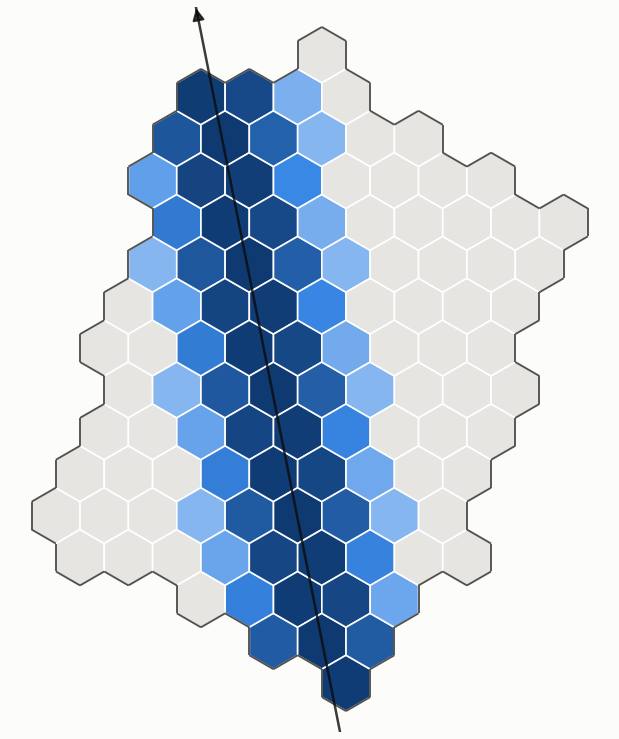
\includegraphics[width=0.48\columnwidth]{concept-river.png}\hfill
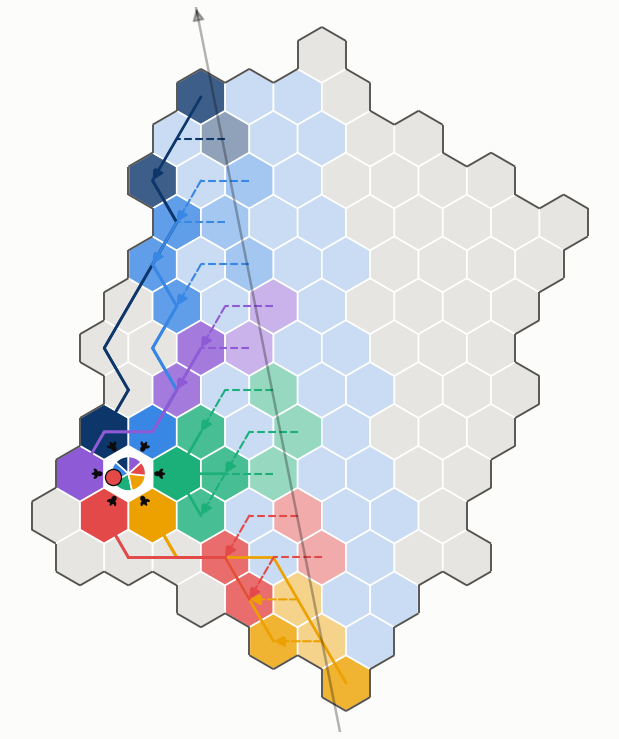
\includegraphics[width=0.48\columnwidth]{concept-circle.png}
\caption{River roles on a cluster with a straight path. Left: \spine{} cells under the path (dark blue), the River band
(lighter towards its edge) and the Banks at the edge. Right: the Ring around a critical cell (red dot); each helper
fetches one group of consecutive segments from the Banks and hands it over in one hop.}\label{fig:roles}
\end{figure}

\begin{algorithm}[t]\caption{River planning at the BS (before take-off)}\label{alg:plan}
\begin{algorithmic}[1]\footnotesize
\REQUIRE path $\gamma$, cluster cells, critical cells $K_c$, range regime
\STATE \spine{} $\leftarrow$ cells crossed by $\gamma$; $\mathrm{Seg}(a)\leftarrow\{s:\gamma(s\Tp)\in a\}$
\FORALL{$a\in$ \spine{}, side $\pm$}
\STATE walk along the local normal of $\gamma$ up to $\omega$ (inner side of a bend: up to the radius of curvature);
$\mathrm{Bank}_\pm(a)\leftarrow$ last cell reached; store the cell path
\ENDFOR
\FORALL{$k\in K_c$}
\STATE $D_k\leftarrow$ the copy of the query emitted nearest to $k$
\STATE helpers $\leftarrow$ 2--12 cells of rings 1--2 around $k$, sized to the predicted lack of $k$
\STATE split \spine{}$\cap D_k$ into consecutive groups; helper $j$ fetches group $j$ from the nearer Banks along
precomputed cell paths
\ENDFOR
\STATE send all tables to the CHs with the flight plan
\end{algorithmic}
\end{algorithm}

\begin{algorithm}[t]\caption{River execution (after the UAV leaves the cluster)}\label{alg:exec}
\begin{algorithmic}[1]\footnotesize
\STATE \textbf{Gather:} in cells with a role, nodes send their CL what the role needs
\STATE \textbf{Bank fill:} a Bank sends a ``have'' manifest of $\mathrm{Seg}(a)$; \spine{} cell $a$ returns what is missing
\STATE \textbf{Repair:} a \spine{} cell completes its segment from adjacent cells; if still incomplete, \textsc{Takeover}
(Algorithm~\ref{alg:takeover})
\STATE \textbf{Ring fill:} helper $j$ requests its group from its Banks
\REPEAT
\STATE \textbf{Final hop:} $k$ sends each helper its lack within the group; the helper forwards packets as they arrive
\UNTIL{$k$ holds $D_k$ (coded: $N'$ packets); a cell idle for 20\,s asks again}
\STATE match and report via the CH
\end{algorithmic}
\end{algorithm}

All steps overlap packet by packet. Requests are ``have'' manifests that fit in one frame. Because the roles depend only
on $\gamma$, River needs no route discovery and no content discovery. With a fountain-coded broadcast the plan is
unchanged except that manifests become counts. The same routes, reversed, let a critical cell pull event crops from the
legacy cameras attached to it; this direction is described in the conference version and not evaluated here.

\textbf{Why it is robust to the range.} River sources data only from the \spine, which receives its own segment whatever
the A2G range. When the range is large it has less to move; when it is small it still completes, whereas schemes that
rely on what a cell hears directly do not.

\subsection{A single-radio lower bound and River's distance from it}
Let $L_k$ be the number of packets of $D_k$ that no node of critical cell $k$ received (its \emph{lack}).
\begin{proposition}\label{prop:radio}
For any ground schedule, critical cell $k$ cannot complete earlier than $\tau_{\min}L_k$ after the UAV has left: every
missing packet must be received by the single radio of its CL over the medium of cell $k$.
\end{proposition}
On 225 critical-cell completions at $R_{50}=99$\,m (experiment of Section~\ref{sec:ground}), cells lack 3744 packets on
average, so the bound is 18\,s. River completes them in 103\,s on average, a median factor 5.1 above the bound; planned
direct pulling is at 5.0 and Deluge at 7.3--7.6 (Fig.~\ref{fig:ground}). A regression over 812 critical cells of 12 runs
(three maps, four regimes) explains where the factor comes from:
\begin{equation}
\widehat T_{\mathrm{River}}(k)=0.71+2.29\,\mathrm{hops}_k+1.97\,\tfrac{L_k}{1000}+4.26\,\tfrac{L_{c(k)}}{1000}\ \text{(s)},\label{eq:surrogate}
\end{equation}
where $\mathrm{hops}_k$ is the cell distance from $k$ to the \spine{} and $L_{c(k)}$ the total lack of the critical cells
of its cluster. A cell's own packets cost about $\tau_f$ each, as the bound predicts, but the packets of the \emph{other}
critical cells of the cluster cost another 4.3\,ms each: the flows share \spine{} cells, Banks and gateways, and each
flow carries its own copy of the same segments. Leave-one-map-out, \eqref{eq:surrogate} has a mean absolute error of
22.8\,s ($R^2=0.60$). Closing the gap to Proposition~\ref{prop:radio} requires forwarding each segment once along a
shared tree instead of once per critical cell; we leave this to future work (Section~\ref{sec:discussion}).

\begin{figure}[t]\centering
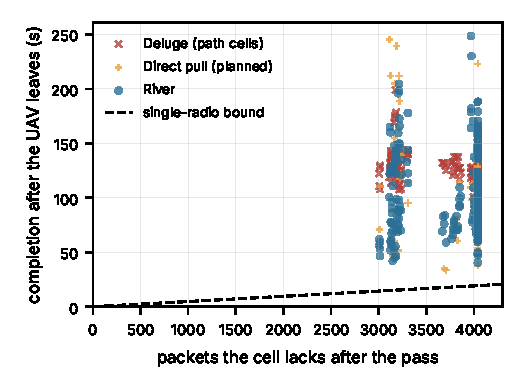
\includegraphics[width=0.82\columnwidth]{ground-lb.pdf}
\caption{Completion time of each critical cell after the UAV has left, against the packets it lacks, for three ground
transports on the same passes (8 clusters, $R_{50}=99$\,m, five network realisations), and the single-radio bound of
Proposition~\ref{prop:radio}.}\label{fig:ground}
\end{figure}

\subsection{Takeover: keeping the plan valid under trajectory error}\label{sec:takeover}
The plan assigns $\mathrm{Seg}(a)$ to \spine{} cell $a$ from the \emph{planned} path. If wind pushes the UAV sideways by
about one reception range, the packets of $\mathrm{Seg}(a)$ are heard by cells that are not adjacent to $a$; the repair
from adjacent cells then fails, and every Bank, Ring and critical cell downstream waits. Takeover restores the segment
without abandoning the plan (Algorithm~\ref{alg:takeover}). Every packet header carries its sequence number and the
position at which it was emitted, so a cell knows which segment a packet belongs to and how far the UAV was from the
planned path.

\begin{algorithm}[t]\caption{\textsc{Takeover} at \spine{} cell $a$ and at a holder cell $c$}\label{alg:takeover}
\begin{algorithmic}[1]\footnotesize
\STATE \textbf{at $a$}, after gathering and the repair from adjacent cells:
\STATE $M\leftarrow\mathrm{Seg}(a)$ minus what $a$ and its adjacent cells hold; \textbf{if} $M=\emptyset$ \textbf{stop}
\STATE $\hat e\leftarrow$ largest distance to the planned path among the emission positions in the headers that $a$ or an
adjacent cell received around $\mathrm{Seg}(a)$
\STATE $h\leftarrow\lceil\hat e/(\sqrt3R_{\mathrm c})\rceil+1$ \ ($h_{\max}$ if no header was received)
\STATE flood \textsc{Query}$(a,M)$ over the cell tree rooted at $a$, $h$ cell hops deep
\STATE \textbf{at $c$}, on \textsc{Query}$(a,M)$: \textbf{if} $c$ holds packets of $M$ that were emitted above $c$ or an
adjacent cell \textbf{then} return them along the reverse path
\STATE \textbf{at $a$}: store the packets; \textbf{if} $M$ is still not covered and $h<h_{\max}$ \textbf{then}
$h\leftarrow h+1$ and flood the new ring
\STATE River continues unchanged: \spine{} $\to$ Bank $\to$ Ring $\to$ critical cell
\end{algorithmic}
\end{algorithm}

Takeover is a repair with respect to an existing plan, not run-time content discovery: when the flight follows the plan
no frame is sent. The following characterises when it is triggered.
\begin{proposition}[Activation]\label{prop:act}
Let $x_s$ be the actual emission position of packet $s$ and $\mathcal N(a)$ the cells adjacent to $a$. Under
independent receptions, takeover is triggered at \spine{} cell $a$ with probability
\begin{equation}
P_{\mathrm{act}}(a)=1-\!\!\prod_{s\in\mathrm{Seg}(a)}\Bigl[1-\!\!\prod_{u\in U_a\cup U_{\mathcal N(a)}}\!\!\bigl(1-p(\lVert x_s-u\rVert)\bigr)\Bigr].\label{eq:act}
\end{equation}
\end{proposition}
On the 840 \spine{} cells of the wind experiment of Section~\ref{sec:wind}, \eqref{eq:act} predicts 2.0, 18.2 and 51.7
activations for deviations of standard deviation 50, 100 and 200\,m; the ns-3 passes show 3, 17 and 48
(Fig.~\ref{fig:act}). Activation rises smoothly with the cross-track deviation $e$ over the segment rather than at a hard
threshold, from below 0.1 for $e<200$\,m to 0.36 at 200--300\,m and 0.92 beyond. Activations at small $e$ are packets that \emph{no} cell
heard, which only a retransmission can repair; activations in which another cell holds the packets---the ones takeover
serves---appear only for $e\ge100$\,m, about one reception range, and never at 50\,m.

\textbf{Query radius.} In the 51 activations with holders, the farthest holder is at most
$\lceil e/(\sqrt3R_{\mathrm c})\rceil+1$ cell hops from $a$, with equality in 9 of them; this is the rule of line~4.
We state it as an empirical rule: a proof needs an assumption on where holders lie, because in the worst direction of
the hexagonal grid one hop covers only $1.5R_{\mathrm c}$. Table~\ref{tab:radius} evaluates the rule offline on the real
pass bitmaps. A fixed radius of 3 hops, as in our ns-3 implementation, reaches all holders at 100\,m but misses two cells
at 200\,m; the adaptive rule with the deviation estimated from received headers reaches 9/9 and 41/42 at its first
attempt while flooding fewer cells than the smallest fixed radius that reaches everything (19.8 against 20.8 cells at
100\,m, 29.7 against 34.0 at 200\,m); the expanding step of line~7 covers the remaining cell.

\begin{figure}[t]\centering
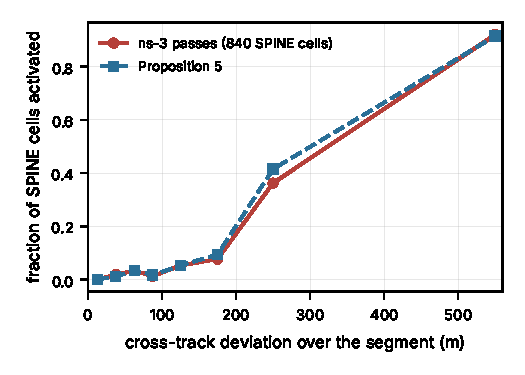
\includegraphics[width=0.8\columnwidth]{propb-activation.pdf}
\caption{Fraction of \spine{} cells in which takeover is triggered versus the cross-track deviation over their segment:
ns-3 passes and Proposition~\ref{prop:act}.}\label{fig:act}
\end{figure}

\begin{table}[t]\centering
\caption{Query radius of takeover, evaluated on the ns-3 wind passes ($R_{50}=99$\,m): activations whose farthest holder
lies inside the flood, and cells flooded per query.}\label{tab:radius}
\footnotesize
\begin{tabular}{lcccc}\toprule
 & \multicolumn{2}{c}{$\sigma=100$\,m (9 activ.)} & \multicolumn{2}{c}{$\sigma=200$\,m (42 activ.)}\\
Rule & reached & cells & reached & cells\\\midrule
fixed 2 hops & 6 & 11.1 & 34 & 13.2\\
fixed 3 hops & 9 & 20.8 & 40 & 23.2\\
fixed 4 hops & 9 & 30.6 & 42 & 34.0\\
adaptive, estimated $\hat e$ & 9 & 19.8 & 41 & 29.7\\
adaptive, true $e$ & 9 & 19.8 & 42 & 29.2\\\bottomrule
\end{tabular}
\end{table}
